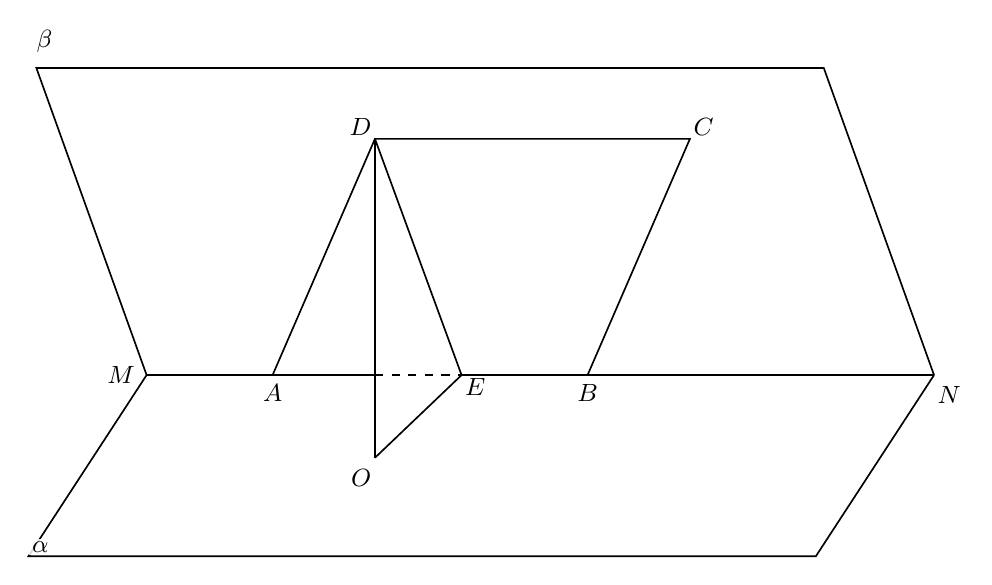
\begin{tikzpicture}[x=1cm,y=1cm,line width=.6pt]
\tikzset{lbl/.style={font=\small,inner sep=1pt,fill=white,fill opacity=0.85,text opacity=1}}
% planes: MN axis
\coordinate (M) at (0,0);
\coordinate (N) at (10,0);
\coordinate (A) at (1.6,0);
\coordinate (E) at (4.0000000000,0.0000000000);
\coordinate (B) at (5.6,0);
\coordinate (D) at (2.9,3.0);
\coordinate (C) at (6.9000000000,3.0000000000);
\coordinate (O) at (2.9000000000,-1.0500000000);
\coordinate (betaL) at (-1.4000000000,3.9000000000);
\coordinate (betaR) at (8.6000000000,3.9000000000);
\coordinate (alphaL) at (-1.5000000000,-2.3000000000);
\coordinate (alphaR) at (8.5000000000,-2.3000000000);
% beta plane outline
\draw (M) -- (betaL) -- (betaR) -- (N);
% alpha plane outline
\draw (M) -- (alphaL) -- (alphaR) -- (N);
% MN ridge
\draw (M)--(2.9,0);\draw[dashed] (2.9,0)--(E);\draw (E)--(N);
% rhombus ABCD in beta
\draw (A) -- (D) -- (C) -- (B);
% triangle DEO: DE solid, DO solid, EO dashed
\draw (D) -- (E);
\draw (D) -- (O);
\draw (E)--(O);
% labels (offset to avoid strokes)
\node[lbl,left=3pt] at (M) {$M$};
\node[lbl,below right,yshift=-3pt] at (N) {$N$};
\node[lbl,below=2pt] at (A) {$A$};
\node[lbl,below right] at (E) {$E$};
\node[lbl,below=2pt] at (B) {$B$};
\node[lbl,above left] at (D) {$D$};
\node[lbl,above right] at (C) {$C$};
\node[lbl,below left,yshift=-3.0pt] at (O) {$O$};
\node[lbl,above left] at ([shift={(0.25,0.15)}]betaL) {$\beta$};
\node[lbl,above right] at (alphaL) {$\alpha$};
\end{tikzpicture}
